\documentclass[
11pt, % The default document font size, options: 10pt, 11pt, 12pt
codirector, % Uncomment to add a codirector to the title page
]{charter} 




% El títulos de la memoria, se usa en la carátula y se puede usar el cualquier lugar del documento con el comando \ttitle
\titulo{Red personalizable de sensores inalámbricos de uso agrícola} 

% Nombre del posgrado, se usa en la carátula y se puede usar el cualquier lugar del documento con el comando \degreename
\posgrado{Carrera de Especialización en Sistemas Embebidos} 
%\posgrado{Carrera de Especialización en Internet de las Cosas} 
%\posgrado{Carrera de Especialización en Intelegencia Artificial}
%\posgrado{Maestría en Sistemas Embebidos} 
%\posgrado{Maestría en Internet de las cosas}

% Tu nombre, se puede usar el cualquier lugar del documento con el comando \authorname
\autor{Ing. Leonardo Agustín Muñoz Valdearenas} 

% El nombre del director y co-director, se puede usar el cualquier lugar del documento con el comando \supname y \cosupname y \pertesupname y \pertecosupname
\director{TBD}
\pertenenciaDirector{TBD} 
% FIXME:NO IMPLEMENTADO EL CODIRECTOR ni su pertenencia
\codirector{TBD} % para que aparezca en la portada se debe descomentar la opción codirector en el documentclass
\pertenenciaCoDirector{TBD}

% Nombre del cliente, quien va a aprobar los resultados del proyecto, se puede usar con el comando \clientename y \empclientename
\cliente{Nicolas Manuel Muñoz}
\empresaCliente{Viña Las Perdices}

% Nombre y pertenencia de los jurados, se pueden usar el cualquier lugar del documento con el comando \jurunoname, \jurdosname y \jurtresname y \perteunoname, \pertedosname y \pertetresname.
\juradoUno{TBD}
\pertenenciaJurUno{TBD} 
\juradoDos{TBD}
\pertenenciaJurDos{TBD}
\juradoTres{TBD}
\pertenenciaJurTres{TBD}
 
\fechaINICIO{20 de junio de 2023}		%Fecha de inicio de la cursada de GdP \fechaInicioName
\fechaFINALPlan{15 de agosto de 2023} 	%Fecha de final de cursada de GdP
\fechaFINALTrabajo{TBD}	%Fecha de defensa pública del trabajo final


\begin{document}

\maketitle
\thispagestyle{empty}
\pagebreak


\thispagestyle{empty}
{\setlength{\parskip}{0pt}
\tableofcontents{}
}
\pagebreak


\section*{Registros de cambios}
\label{sec:registro}


\begin{table}[ht]
\label{tab:registro}
\centering
\begin{tabularx}{\linewidth}{@{}|c|X|c|@{}}
\hline
\rowcolor[HTML]{C0C0C0} 
Revisión & \multicolumn{1}{c|}{\cellcolor[HTML]{C0C0C0}Detalles de los cambios realizados} & Fecha      \\ \hline
0      & Creación del documento                                 &\fechaInicioName \\ \hline
1      & Se completa hasta el punto 5 inclusive                 & 4 de julio de 2023 \\ \hline
2      & Se completa hasta el punto 9 inclusive					& 12 de julio de 2023 \\ \hline
3      & Se completa hasta el punto 12 inclusive				& 25 de julio de 2023 \\ \hline
%		  Se puede agregar algo más \newline
%		  En distintas líneas \newline
%		  Así                                                    & dd/mm/aaaa \\ \hline
%3      & Se completa hasta el punto 11 inclusive                & dd/mm/aaaa \\ \hline
%4      & Se completa el plan	                                 & dd/mm/aaaa \\ \hline
\end{tabularx}
\end{table}

\pagebreak



\section*{Acta de constitución del proyecto}
\label{sec:acta}

\begin{flushright}
Buenos Aires, \fechaInicioName
\end{flushright}

\vspace{2cm}

Por medio de la presente se acuerda con el \authorname\hspace{1px} que su Trabajo Final de la \degreename\hspace{1px} se titulará ``\ttitle'', consistirá esencialmente en el desarrollo de una red de sensores distribuida para la medición de parámetros ambientales, y tendrá un presupuesto preliminar estimado de 625 h de trabajo y \textcolor{red}{\$800.000}, con fecha de inicio \fechaInicioName\hspace{1px} y fecha de presentación pública \fechaFinalName.

Se adjunta a esta acta la planificación inicial.

\vfill

% Esta parte se construye sola con la información que hayan cargado en el preámbulo del documento y no debe modificarla
\begin{table}[ht]
\centering
\begin{tabular}{ccc}
\begin{tabular}[c]{@{}c@{}}Dr. Ing. Ariel Lutenberg \\ Director posgrado FIUBA\end{tabular} & \hspace{2cm} & \begin{tabular}[c]{@{}c@{}}\clientename \\ \empclientename \end{tabular} \vspace{2.5cm} \\ 
\multicolumn{3}{c}{\begin{tabular}[c]{@{}c@{}} \supname \\ Director del Trabajo Final\end{tabular}} \vspace{2.5cm} \\
%\begin{tabular}[c]{@{}c@{}}\jurunoname \\ Jurado del Trabajo Final\end{tabular}     &  & \begin{tabular}[c]{@{}c@{}}\jurdosname\\ Jurado del Trabajo Final\end{tabular}  \vspace{2.5cm}  \\
%\multicolumn{3}{c}{\begin{tabular}[c]{@{}c@{}} \jurtresname\\ Jurado del Trabajo Final\end{tabular}} \vspace{.5cm}                                                                     
\end{tabular}
\end{table}




\section{1. Descripción técnica-conceptual del proyecto a realizar}
\label{sec:descripcion}

En la actualidad, se observa una tendencia en alza hacia el monitoreo de parámetros en los procesos productivos en general. El propósito de esta práctica es incrementar los rendimientos, reducir el consumo de recursos y optimizar los resultados obtenidos. Esto puede extrapolarse al sector agrícola, donde la medición de parámetros involucrados en el desarrollo del fruto, tales como temperatura y humedad del sueldo, ayuda a mejorar la calidad el producto final obtenido. Las principales ventajas del monitoreo y control de cultivos mediante este tipo de técnicas son:

\begin{itemize}
\item Ahorro de agua de riego.
\item Prevención de enfermedades.
\item Detección de falencias en el sistema de riego.
\item Identificación de zonas dañadas por heladas.
\item Uso eficiente de agroquímicos.
\end{itemize}

Para la medición de los parámetros que el cliente requiera, se deben distribuir sensores con su correspondiente microcontrolador y sistema de energía autónomo, usualmente basado en energía solar. Una vez los sensores fueron distribuidos, la recolección de datos se puede realizar de dos diferentes maneras en términos generales:

\begin{itemize}
\item Recolección manual: en este esquema los nodos sensores registran las mediciones en una memoria interna y el usuario debe extraer dichas mediciones periodicamente de manera manual. Si bien es una solución sencilla y de bajo costo, su desventaja principal es su imposibilidad de uso en ubicaciones remotas de difícil acceso.

\item Recolección mediante punto de acceso: otra manera de obtener las mediciones de los sensores distribuidos es mediante una conexión a internet a través de un punto de acceso (o usualmente llamado gateway), de esta manera los datos son accesibles para el usuario de manera remota por medio de una base de datos. Este concepto de utilizar un punto de acceso a internet es lo que hoy se conoce como internet de la cosas (IoT de sus siglas en inglés). Es evidente que un esquema de este estilo mejora de manera significativa la experiencia de usuario de acceso los datos, aunque implica una mayor complejidad por la necesidad de mantener activo un enlace de comunicaciones y eventualmente requerir algún mantenimiento.
\end{itemize}

En este proyecto se propone la utilización del segundo esquema de recolección de datos planteado previamente, aunque reemplazando el acceso a internet de un único sensor por una red de sensores inalámbrica (WSN de sus siglas en ingles Wireless Sensor Network) con único punto de acceso a internet como puede observarse a continuación en la figura \ref{fig:WSN_architecture}.

\begin{figure}[htpb]
\centering 
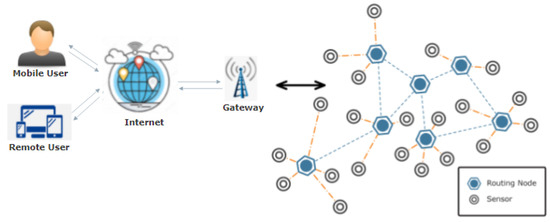
\includegraphics[width=1\textwidth]{./Figuras/WSN_architecture.jpg}
\caption{Arquitectura de una WSN.}
\label{fig:WSN_architecture}
\end{figure}

La implementación WSN se ha visto disminuida en costos, principalmente por los avances tecnológicos en lo que respecta a capacidad de integración y disminución de consumo, permitiendo la llegada a un mercado masivo.

El propósito del desarrollo de una WSN como plataforma en sí, es permitir al cliente en particular elegir los parámetros que desea medir en sus cultivos y así dar una mayor personalización en la solución, por ejemplo, si se desease medir el valor de pH de una zona en particular con un sensor que el cliente requiera, este podría adaptarse de manera casi transparente para la red. Además, permite una generalización en el diseño ya que se parte de una base común que abarca la implementación de la red y los protocolos, permitiendo una fácil adaptación a los requerimientos de cada cliente.

Bajo este esquema, el proyecto requerirá del desarrollo de tres módulos principales como se observa en la figura \ref{fig:DiagramaGeneral} y la función de cada uno de estos se lista a continuación:

\begin{itemize}
\item Nodo con punto de acceso o gateway: es el nodo encargado de la recepción de los datos de toda la red (siguiendo un esquema de red mesh), y enviarlos a internet para que estén disponibles para el usuario. Además almacenará los datos de manera local en caso de que hubiese una falla con el enlace.
\item Nodo de enrutamiento: su función es colectar de los datos de los nodos sensores que este tenga conectados y rediccionar mensajes de otros nodos de enrutamiento dentro de la red, para que los mismos puedan llegar al nodo con punto de acceso.
\item Nodo sensor: es el nodo encargado de la adquisición periódica de los datos del sensor que este tenga conectado y su envío hacia el nodo de enrutamiento más cercano.
\end{itemize}

\begin{figure}[H]
\centering 
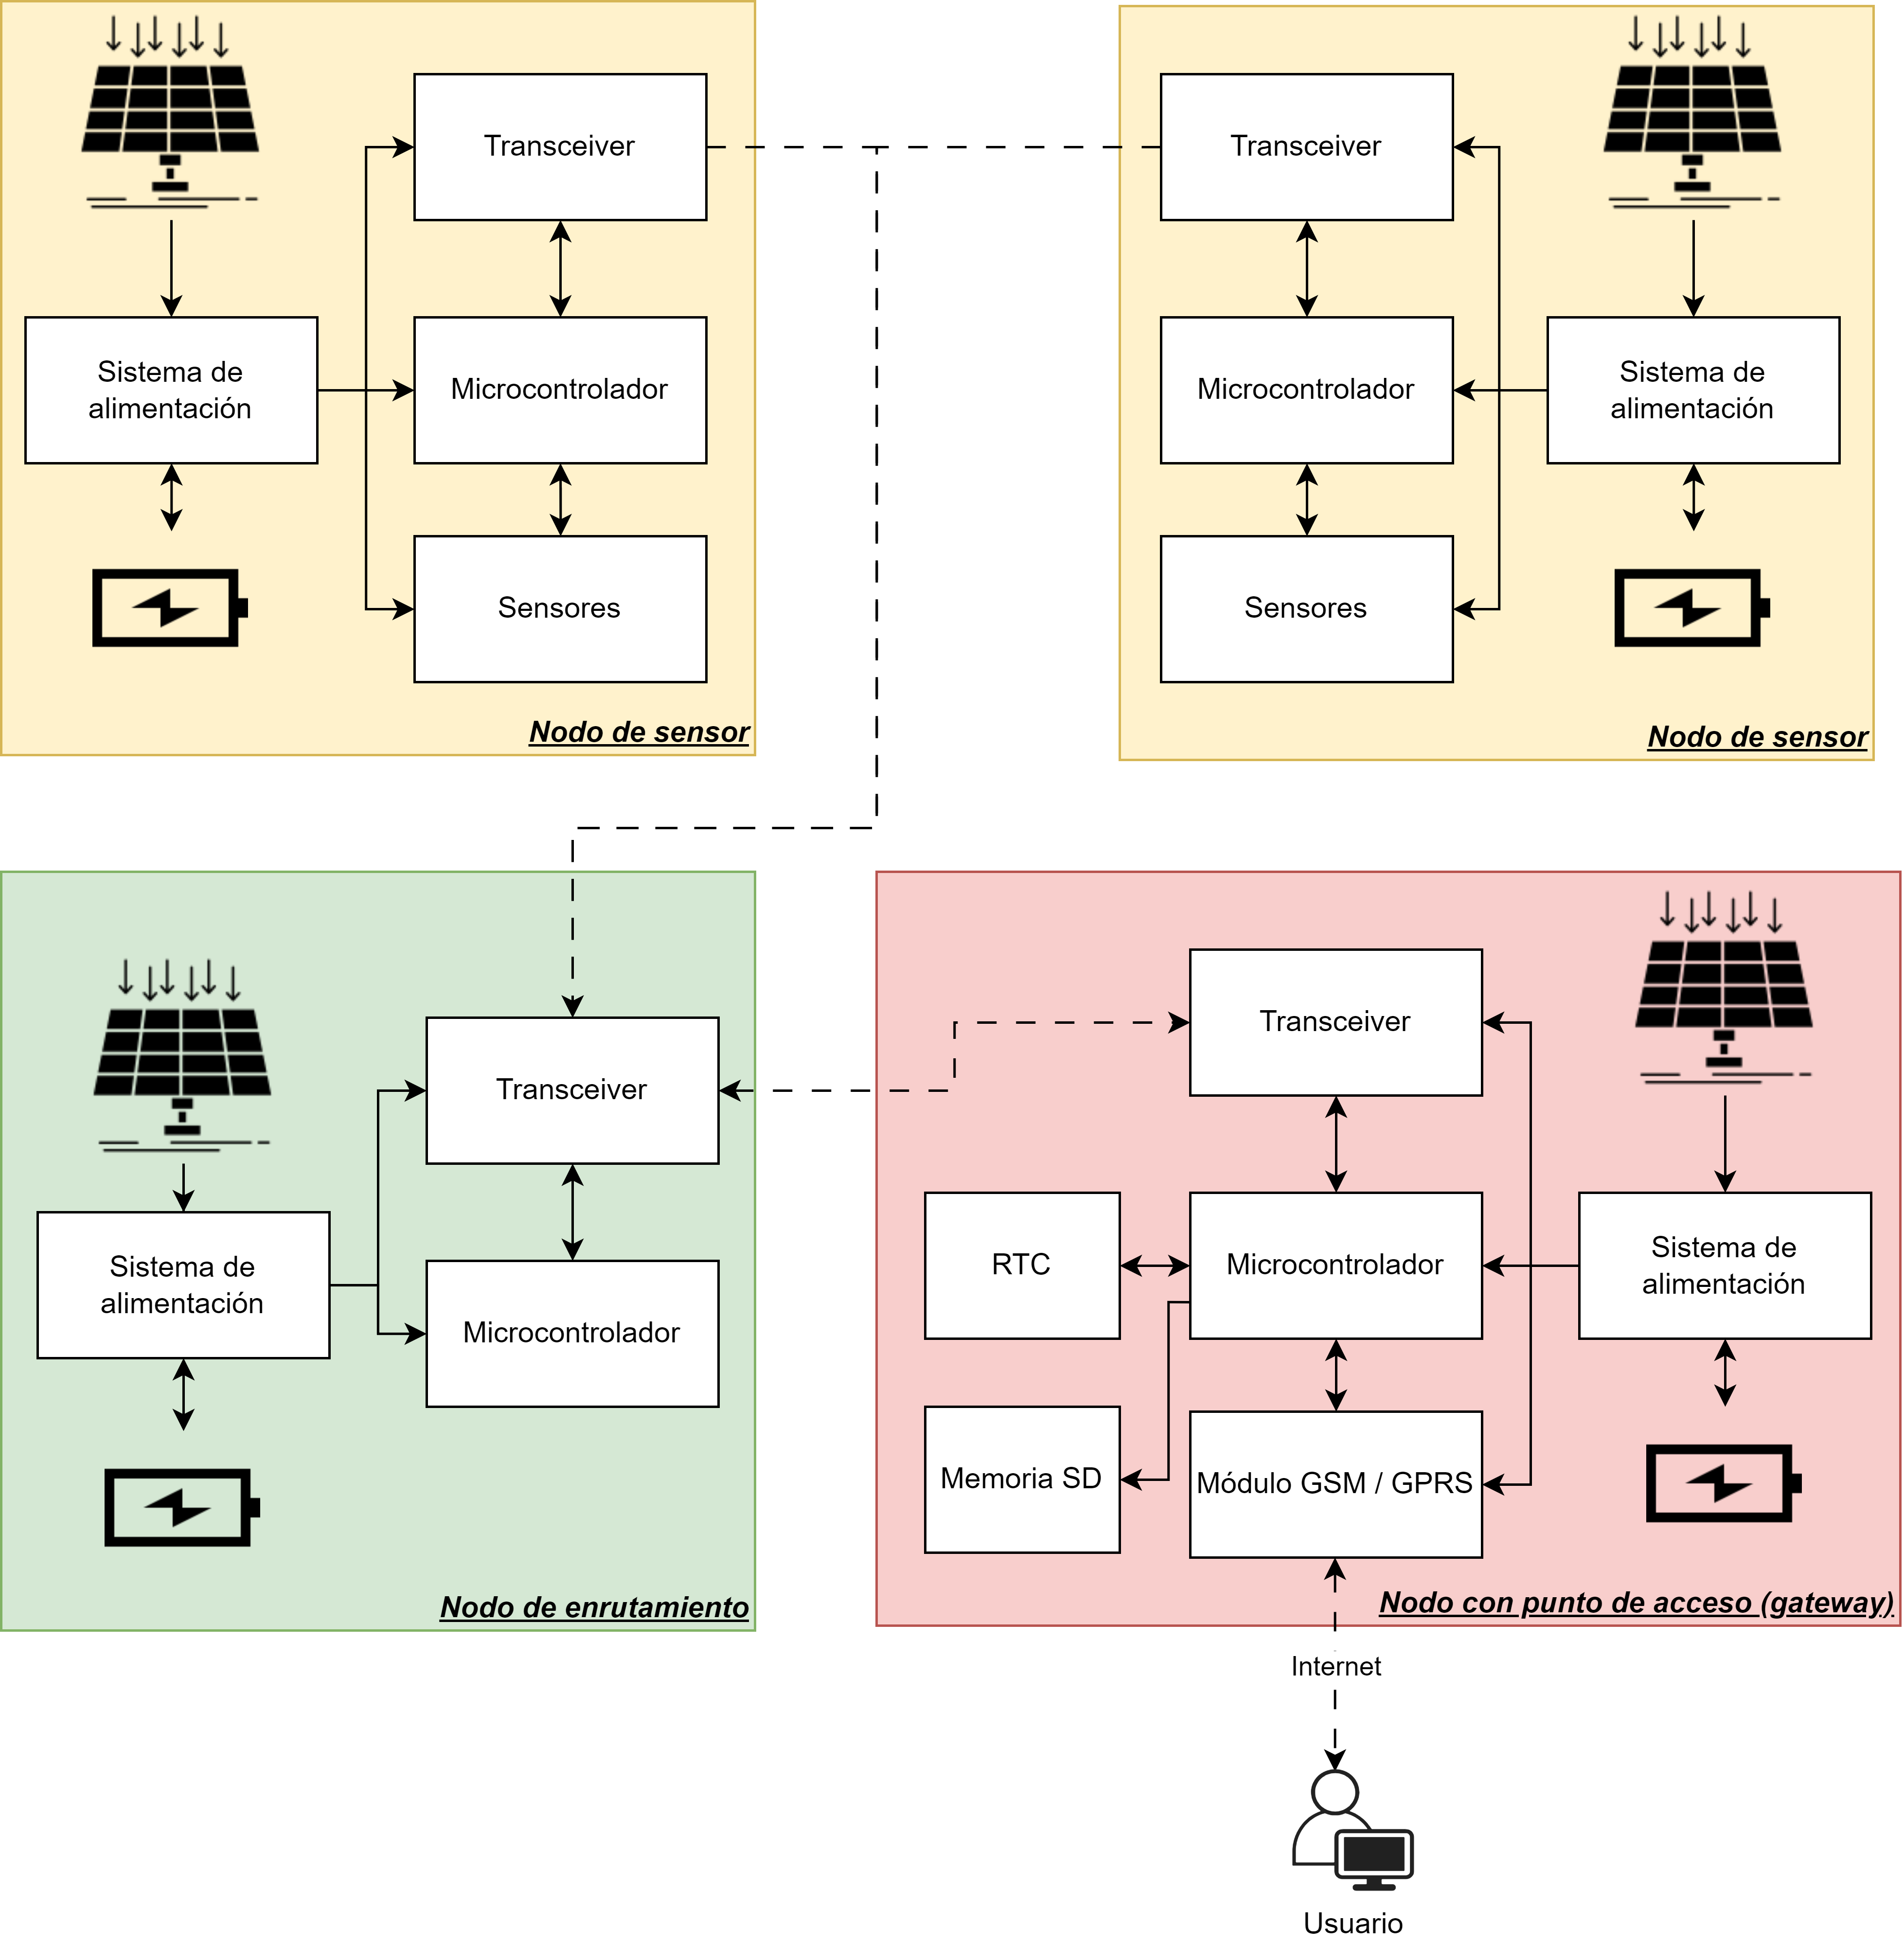
\includegraphics[width=.9\textwidth]{./Figuras/DiagramaGeneral.png}
\caption{Diagrama general de la red WSN propuesta.}
\label{fig:DiagramaGeneral}
\end{figure}


En la actualidad existen diferentes tecnologías para el transceiver que se encuentra dentro de los módulos mencionados previamente. Estas se diferencian principalmente en lo que refiere a consumo, tasa de datos, cantidad de dispositivos que admite, distancia máxima de comunicación y el costo final por nodo de comunicación. Las más utilizadas se listan a continuación:

\begin{itemize}
\item Bluetooth de bajo consumo.
\item LoraWAN.
\item Narrow Band IoT.
\item Sigfox.
\item 6LoWPAN.
\item Wi-Fi.
\item Zigbee.
\end{itemize}

Es importante aclarar que la definición del tipo de transceiver utilizado en el presente proyecto se realizará durante el desarrollo el proyecto. A modo de análisis preliminar, debe optarse por una opción que priorice el bajo consumo por sobre una alta tasa de datos ya que en aplicaciones agrícolas los parámetros a analizar son en general de variación lenta. Además, se prevé una distancia entre nodos sensores del orden de decenas de metros en lugar de kilómetros, por lo que una tecnología de gran alcance no resulta algo prioritario.

\section{2. Identificación y análisis de los interesados}
\label{sec:interesados}

\begin{table}[ht]
%\caption{Identificación de los interesados}
%\label{tab:interesados}
\begin{tabularx}{\linewidth}{@{}|l|X|X|l|@{}}
\hline
\rowcolor[HTML]{C0C0C0} 
Rol           & Nombre y Apellido & Organización 	& Puesto 	\\ \hline
Cliente       & \clientename      &\empclientename	& Apoderado  \\ \hline
Responsable   & \authorname       & FIUBA        	& Alumno 	\\ \hline
Orientador    & \supname	      & \pertesupname 	& Director Trabajo final \\ \hline
Usuario final & Ing. Christian Ciaglo &\empclientename & Ing. Agrónomo\\ \hline
\end{tabularx}
\end{table}

Las características principales de cada uno de los interesados listados previamente son:

\begin{itemize}
\item \clientename : persona entusiasta, fomenta la inversión en nuevas tecnologías dentro de su empresa pero siempre que se demuestre fehasientemente que la inversión será rentable. Como cualquier persona con un cargo gerencial, dispone de poco tiempo por lo que los resultados deben ser concisos y comprobables.
\item Director : aún sin definir.
\item Ing. Christian Ciaglo : ingeniero agrónomo a cargo del cuidado del viñedo de la bodega, actualmente tiene instalados sensores del estilo de recolección manual (como se categorizó en la sección \ref{sec:descripcion}). Es la persona que ayudará a establecer los requerimientos de los sensores y será el principal beneficiario de los resultados del proyecto, por lo que es de gran importancia mantener una comunicación periódica durante la etapa temprana del proyecto.
\end{itemize}

\section{3. Propósito del proyecto}
\label{sec:proposito}

El propósito de este proyecto es el desarrollo de una red de sensores distribuidos de bajo costo y con gran escalabilidad, para que los productores dispongan de datos de alta resolución espacial que mejoren la toma de decisiones, aumentando así ganancias y rendimientos de sus cultivos. Esto se propone tomando como base que la mayoría de la matriz productiva Argentina depende del sector agrícola en general. A pesar de esto, un porcentaje muy pequeño de productores disponen de métricas ambientales y de salud de sus cultivos, lo cual podría incrementar el rendimiento de sus cultivos de manera significativa. Esto puede deberse a falta de interés por su conocimiento, baja oferta de soluciones en el mercado o bien porque se requiere de una gran inversión inicial.

\section{4. Alcance del proyecto}
\label{sec:alcance}

Como se especificó en la sección \ref{sec:descripcion}, el proyecto requiere del desarrollo de tres módulos principales y una interfaz de usuario para la visualización e interpretación de los datos colectados. En lo que refiere a la presentación de proyecto dentro del marco de la \degreename, no se realizará un software de visualización específico, sino que se adaptará a la utilización de algún software previamente desarrollado que cumpla los requerimientos propuestos.

Se realizará una fabricación de una cantidad de módulos limitada pero suficientes para validar el funcionamiento integral del proyecto propuesto, por lo que no se realizará un lote de producción en serie que afecte la duración del proyecto.

\section{5. Supuestos del proyecto}
\label{sec:supuestos}

Para el desarrollo del presente proyecto se toman en cuenta los siguientes supuestos que refieren al marco de desarrollo:

\begin{itemize}
\item Disponibilidad de componentes: si bien en este proyecto se realizará un gran esfuerzo por priorizar el uso de componentes disponibles a nivel nacional, inevitablemente habrán componentes específicos dentro del diseño que deberán ser adquiridos desde el exterior.
\item Políticas macroeconómicas: se supondrá que las políticas de importación se mantendrán como lo hacen actualmente, lo cual permite el ingreso al país de pequeñas cantidades de componentes sin necesidad de presentar una excesiva cantidad de documentación legal que pueda afectar los tiempos de desarrollo del proyecto.
\item Desarrollo a nivel prototipo: este proyecto solo será fabricado a nivel de prototipo sin realizar iteraciones para optimizar la producción en serie del mismo.
\item Permiso de comunicaciones: para la comunicaciones dentro de la WSN se utilizará una banda no licenciada para evitar la necesidad de permisos especiales, en caso de que ocurra un cambio legal durante el desarrollo del proyecto se tomará una decisión conjunta con las autoridades del proyecto para evaluar que la alternativa no perjudique de manera significativa el desarrollo del proyecto.
\end{itemize}

\section{6. Requerimientos}
\label{sec:requerimientos}

\begin{enumerate}
	\item Requerimientos funcionales
	
		\begin{enumerate}
		
			\item Comunicaciones.
			\begin{enumerate}
				\item Se debe usar una frecuencia de uso no licenciado.
				\item En cada red debe haber solamente un único nodo gateway.
				\item El nodo gateway debe enviar los datos a internet mediante la red celular.
				\item Cada módulo debe tener un identificador único.
				\item Se debe implementar un protocolo de comunicación con confirmación de recepción de paquetes.
				\item Los módulos debe tener un indicador lumínico para indicar errores.
			\end{enumerate}
			
			\item Alimentación.
			\begin{enumerate}
				\item Los módulos deben disponer de un panel solar.
				\item Los módulos deben almacenar energía en una batería.
				\item Todos los módulos deben enviar el porcentaje de batería restante de forma periódica.
				\item La vida útil de la batería debe ser mayor a 10 años.
			\end{enumerate}
			
			\item Datos.
			\begin{enumerate}
				\item Cada nodo envía una única medición por trama.
				\item El nodo gateway debe tener una memoria auxiliar donde almacene los datos.
				\item El nodo gateway debe colocar una estampa de tiempo a los datos.
			\end{enumerate}
			
		\end{enumerate}
	\item Requerimientos de documentación.
		\begin{enumerate}
			\item Se debe documentar de manera clara el protocolo de comunicación.
			\item Los formatos de trama deben estar claramente documentados.
			\item Se deberá justificar el dimensionamiento del sistema de alimentación de cada tipo de módulo.
			\item Se deberán documentar procedimientos de puesta en marcha de los módulos.
			\item Se deberá realizar un informe de avance del proyecto y una memoria de trabajo final, una vez finalizado el mismo.
		\end{enumerate}

	\item Requerimientos de testing.
		\begin{enumerate}
			\item Se deben presentar resultados de cobertura de las pruebas unitarias y de integración.
			\item Se deben realizar pruebas de aceptación en presencia del cliente.
			\item Se deben evidenciar los resultados obtenidos en las pruebas de sistema.
		\end{enumerate}

	\item Requerimientos de interoperatividad.
		\begin{enumerate}
			\item Los datos enviados a internet deben tener un formato JSON, de tal forma de ser compatible con interfaces de usuario desarrolladas por terceros.
		\end{enumerate}
					
\end{enumerate}

\section{7. Historias de usuarios (\textit{Product backlog})}
\label{sec:backlog}

A continuación se muestra el puntaje que se asignará a cada item dentro de los \textit{story points}:

\begin{enumerate}
	\item Dificultad.
	\begin{itemize}
		\item Baja 2.
		\item Media 5.
		\item Alta 13.
	\end{itemize}

\item Complejidad.
	\begin{itemize}
		\item Baja 5.
		\item Media 8.
		\item Alta 13.
	\end{itemize}

\item Riesgo.
	\begin{itemize}
		\item Baja 1.
		\item Media 3.
		\item Alta 8.
	\end{itemize}
\end{enumerate}


Como cliente quiero que la cantidad de módulos pueda escalarse para cubrir la superficie de todo el viñedo.
\begin{itemize}
\item Dificultad media (5): lograr establecer numerosos enlaces de radio de baja potencia y de manera simultánea en una gran extensión no es una tarea trivial, aunque no se espera que sea de gran dificultad. 
\item Complejidad alta (13): requerirá la implementación de un protocolo de comunicación lo suficientemente robusto para establecer cientos de enlaces, por lo que complejizará significativamente el esquema de acceso al medio.
\item Riesgo alto (8): en caso de que esto no pueda lograrse, significaría un gran fracaso en el proyecto y requeriría de un replanteamiento de hardware y de la topología de la red.
\end{itemize}
\textit{Story point}: 34.

Como usuario quiero que los nodos sensores sean versátiles para poder probar diferentes sensores y poder experimentar en función de los resultados.
\begin{itemize}
\item Dificultad baja (2): los sensores comerciales en su mayoría utilizan interfaces de comunicación estándar, por lo que se prevé que la integración de estos sea relativamente sencilla.
\item Complejidad media (8): se requerirá implementar el driver para el sensor en particular (tramas, tasa de datos, control de errores, etc.).
\item Riesgo medio (3): en caso de que no pueda realizarse la adapatación directa con algún sensor específico, se espera que las horas de ingeniería para adaptarlo a la plataforma sean bajas.
\end{itemize}
\textit{Story point}: 13.

\section{8. Entregables principales del proyecto}
\label{sec:entregables}

Los entregables del proyecto son:

\begin{itemize}
	\item Un prototipo del nodo gateway.
	\item Dos prototipos del nodo de enrutamiento.
	\item Cuatro prototipos del nodo sensor.
	\item Circuitos esquemáticos.
	\item Código fuente del firmware.
	\item Intrucciones de puesta en marcha.
	\item Manual de usuario.
	\item Informe final.
\end{itemize}


\section{9. Desglose del trabajo en tareas}
\label{sec:wbs}

A continuación se presenta el desglose de trabajo en tareas con su correspondiente duración estimada:

\begin{enumerate}
\item Desarrollo de módulos.

	\begin{enumerate}
	
	\item Enlace de comunicación (subtotal 160 h).
		\begin{enumerate}
			\item Implementación del protocolo dentro de la WSN (30 h).
			\item Desarrollo del método de enrutamiento automático (30 h).
			\item Definición del formato de tramas (15 h).
			\item Desarrollo de la interfaz con el transceiver (40 h).
			\item Realizar control de paquetes (25 h).
			\item Desarrollo de la interfaz con módulo de red celular (20 h).
			
		\end{enumerate}
		
	\item Alimentación (subtotal 55 h).
	
		\begin{enumerate}
			\item Estimación y verificación de consumos (10 h).
			\item Dimensionamiento de componentes (15 h).
			\item Selección de componentes (30 h).
			
		\end{enumerate}
		
	\item Sensores (subtotal 60 h).
	
		\begin{enumerate}
			\item Selección de sensores (20 h).
			\item Programación de drivers específicos (40 h).
		\end{enumerate}
	
	\item Armado (subtotal 130 h).
	
		\begin{enumerate}
			\item Diseño de esquemáticos (40 h).
			\item Armado y prueba del prototipo (20 h).
			\item Diseño de placas (40 h).
			\item Ensamblaje de módulos definitivos (30 h).
		
		\end{enumerate}
		
	\end{enumerate}
	
\item Testing (subtotal 90 h).
	\begin{enumerate}
	\item Realizar pruebas unitarias (40 h).
	\item Realizar pruebas de integración (25 h).
	\item Realizar pruebas de sistema (25 h).
	\end{enumerate}
	
\item Documentación (subtotal 130 h).
	\begin{enumerate}
	\item Realizar reporte de testing (30 h).
	\item Redacción del manual de usuario (20 h).
	\item Elaboración del informe de avance (20 h).
	\item Redacción de la memoria de trabajo final (40 h).
	\item Elaboración de la presentación de proyecto (20 h).
	\end{enumerate}
	
\end{enumerate}

Total de horas del proyecto: 625 h.

\section{10. Diagrama de Activity On Node}
\label{sec:AoN}

\begin{consigna}{red}
Armar el AoN a partir del WBS definido en la etapa anterior. 

%La figura \ref{fig:AoN} fue elaborada con el paquete latex tikz y pueden consultar la siguiente referencia \textit{online}:

%\url{https://www.overleaf.com/learn/latex/LaTeX_Graphics_using_TikZ:_A_Tutorial_for_Beginners_(Part_3)\%E2\%80\%94Creating_Flowcharts}

\end{consigna}

\begin{figure}[htpb]
\centering 
\includegraphics[width=.8\textwidth]{./Figuras/AoN.png}
\caption{Diagrama de \textit{Activity on Node}.}
\label{fig:AoN}
\end{figure}

Indicar claramente en qué unidades están expresados los tiempos.
De ser necesario indicar los caminos semicríticos y analizar sus tiempos mediante un cuadro.
Es recomendable usar colores y un cuadro indicativo describiendo qué representa cada color, como se muestra en el siguiente ejemplo:



\section{11. Diagrama de Gantt}
\label{sec:gantt}

\begin{consigna}{red}

Existen muchos programas y recursos \textit{online} para hacer diagramas de Gantt, entre los cuales destacamos:

\begin{itemize}
\item Planner
\item GanttProject
\item Trello + \textit{plugins}. En el siguiente link hay un tutorial oficial: \\ \url{https://blog.trello.com/es/diagrama-de-gantt-de-un-proyecto}
\item Creately, herramienta online colaborativa. \\\url{https://creately.com/diagram/example/ieb3p3ml/LaTeX}
\item Se puede hacer en latex con el paquete \textit{pgfgantt}\\ \url{http://ctan.dcc.uchile.cl/graphics/pgf/contrib/pgfgantt/pgfgantt.pdf}
\end{itemize}

Pegar acá una captura de pantalla del diagrama de Gantt, cuidando que la letra sea suficientemente grande como para ser legible. 
Si el diagrama queda demasiado ancho, se puede pegar primero la ``tabla'' del Gantt y luego pegar la parte del diagrama de barras del diagrama de Gantt.

Configurar el software para que en la parte de la tabla muestre los códigos del EDT (WBS).\\
Configurar el software para que al lado de cada barra muestre el nombre de cada tarea.\\
Revisar que la fecha de finalización coincida con lo indicado en el Acta Constitutiva.

En la figura \ref{fig:gantt}, se muestra un ejemplo de diagrama de Gantt realizado con el paquete de \textit{pgfgantt}. En la plantilla pueden ver el código que lo genera y usarlo de base para construir el propio.

\begin{figure}[htbp]
\begin{center}
\begin{ganttchart}{1}{12}
  \gantttitle{2020}{12} \\
  \gantttitlelist{1,...,12}{1} \\
  \ganttgroup{Group 1}{1}{7} \\
  \ganttbar{Task 1}{1}{2} \\
  \ganttlinkedbar{Task 2}{3}{7} \ganttnewline
  \ganttmilestone{Milestone o hito}{7} \ganttnewline
  \ganttbar{Final Task}{8}{12}
  \ganttlink{elem2}{elem3}
  \ganttlink{elem3}{elem4}
\end{ganttchart}
\end{center}
\caption{Diagrama de Gantt de ejemplo}
\label{fig:gantt}
\end{figure}


\begin{landscape}
\begin{figure}[htpb]
\centering 
\includegraphics[height=.85\textheight]{./Figuras/Gantt-2.png}
\caption{Ejemplo de diagrama de Gantt rotado}
\label{fig:diagGantt}
\end{figure}

\end{landscape}

\end{consigna}


\section{12. Presupuesto detallado del proyecto}
\label{sec:presupuesto}

\begin{consigna}{red}
Si el proyecto es complejo entonces separarlo en partes:
\begin{itemize}
	\item Un total global, indicando el subtotal acumulado por cada una de las áreas.
	\item El desglose detallado del subtotal de cada una de las áreas.
\end{itemize}

IMPORTANTE: No olvidarse de considerar los COSTOS INDIRECTOS.

\end{consigna}

\begin{table}[htpb]
\centering
\begin{tabularx}{\linewidth}{@{}|X|c|r|r|@{}}
\hline
\rowcolor[HTML]{C0C0C0} 
\multicolumn{4}{|c|}{\cellcolor[HTML]{C0C0C0}COSTOS DIRECTOS} \\ \hline
\rowcolor[HTML]{C0C0C0} 
Descripción &
  \multicolumn{1}{c|}{\cellcolor[HTML]{C0C0C0}Cantidad} &
  \multicolumn{1}{c|}{\cellcolor[HTML]{C0C0C0}Valor unitario} &
  \multicolumn{1}{c|}{\cellcolor[HTML]{C0C0C0}Valor total} \\ \hline
 &
  \multicolumn{1}{c|}{} &
  \multicolumn{1}{c|}{} &
  \multicolumn{1}{c|}{} \\ \hline
 &
  \multicolumn{1}{c|}{} &
  \multicolumn{1}{c|}{} &
  \multicolumn{1}{c|}{} \\ \hline
\multicolumn{1}{|l|}{} &
   &
   &
   \\ \hline
\multicolumn{1}{|l|}{} &
   &
   &
   \\ \hline
\multicolumn{3}{|c|}{SUBTOTAL} &
  \multicolumn{1}{c|}{} \\ \hline
\rowcolor[HTML]{C0C0C0} 
\multicolumn{4}{|c|}{\cellcolor[HTML]{C0C0C0}COSTOS INDIRECTOS} \\ \hline
\rowcolor[HTML]{C0C0C0} 
Descripción &
  \multicolumn{1}{c|}{\cellcolor[HTML]{C0C0C0}Cantidad} &
  \multicolumn{1}{c|}{\cellcolor[HTML]{C0C0C0}Valor unitario} &
  \multicolumn{1}{c|}{\cellcolor[HTML]{C0C0C0}Valor total} \\ \hline
\multicolumn{1}{|l|}{} &
   &
   &
   \\ \hline
\multicolumn{1}{|l|}{} &
   &
   &
   \\ \hline
\multicolumn{1}{|l|}{} &
   &
   &
   \\ \hline
\multicolumn{3}{|c|}{SUBTOTAL} &
  \multicolumn{1}{c|}{} \\ \hline
\rowcolor[HTML]{C0C0C0}
\multicolumn{3}{|c|}{TOTAL} &
   \\ \hline
\end{tabularx}%
\end{table}


\section{13. Gestión de riesgos}
\label{sec:riesgos}

\begin{consigna}{red}
a) Identificación de los riesgos (al menos cinco) y estimación de sus consecuencias:
 
Riesgo 1: detallar el riesgo (riesgo es algo que si ocurre altera los planes previstos de forma negativa)
\begin{itemize}
	\item Severidad (S): mientras más severo, más alto es el número (usar números del 1 al 10).\\
	Justificar el motivo por el cual se asigna determinado número de severidad (S).
	\item Probabilidad de ocurrencia (O): mientras más probable, más alto es el número (usar del 1 al 10).\\
	Justificar el motivo por el cual se asigna determinado número de (O). 
\end{itemize}   

Riesgo 2:
\begin{itemize}
	\item Severidad (S): 
	\item Ocurrencia (O):
\end{itemize}

Riesgo 3:
\begin{itemize}
	\item Severidad (S): 
	\item Ocurrencia (O):
\end{itemize}


b) Tabla de gestión de riesgos:      (El RPN se calcula como RPN=SxO)

\begin{table}[htpb]
\centering
\begin{tabularx}{\linewidth}{@{}|X|c|c|c|c|c|c|@{}}
\hline
\rowcolor[HTML]{C0C0C0} 
Riesgo & S & O & RPN & S* & O* & RPN* \\ \hline
       &   &   &     &    &    &      \\ \hline
       &   &   &     &    &    &      \\ \hline
       &   &   &     &    &    &      \\ \hline
       &   &   &     &    &    &      \\ \hline
       &   &   &     &    &    &      \\ \hline
\end{tabularx}%
\end{table}

Criterio adoptado: 
Se tomarán medidas de mitigación en los riesgos cuyos números de RPN sean mayores a...

Nota: los valores marcados con (*) en la tabla corresponden luego de haber aplicado la mitigación.

c) Plan de mitigación de los riesgos que originalmente excedían el RPN máximo establecido:
 
Riesgo 1: plan de mitigación (si por el RPN fuera necesario elaborar un plan de mitigación).
  Nueva asignación de S y O, con su respectiva justificación:
  - Severidad (S): mientras más severo, más alto es el número (usar números del 1 al 10).
          Justificar el motivo por el cual se asigna determinado número de severidad (S).
  - Probabilidad de ocurrencia (O): mientras más probable, más alto es el número (usar del 1 al 10).
          Justificar el motivo por el cual se asigna determinado número de (O).

Riesgo 2: plan de mitigación (si por el RPN fuera necesario elaborar un plan de mitigación).
 
Riesgo 3: plan de mitigación (si por el RPN fuera necesario elaborar un plan de mitigación).

\end{consigna}


\section{14. Gestión de la calidad}
\label{sec:calidad}

\begin{consigna}{red}
Elija al menos diez requerientos que a su criterio sean los más importantes/críticos/que aportan más valor y para cada uno de ellos indique las acciones de verificación y validación que permitan asegurar su cumplimiento.

\begin{itemize} 
\item Req \#1: copiar acá el requerimiento.

\begin{itemize}
	\item Verificación para confirmar si se cumplió con lo requerido antes de mostrar el sistema al cliente. Detallar 
	\item Validación con el cliente para confirmar que está de acuerdo en que se cumplió con lo requerido. Detallar  
\end{itemize}

\end{itemize}

Tener en cuenta que en este contexto se pueden mencionar simulaciones, cálculos, revisión de hojas de datos, consulta con expertos, mediciones, etc.  Las acciones de verificación suelen considerar al entregable como ``caja blanca'', es decir se conoce en profundidad su funcionamiento interno.  En cambio, las acciones de validación suelen considerar al entregable como ``caja negra'', es decir, que no se conocen los detalles de su funcionamiento interno.

\end{consigna}

\section{15. Procesos de cierre}    
\label{sec:cierre}

\begin{consigna}{red}
Establecer las pautas de trabajo para realizar una reunión final de evaluación del proyecto, tal que contemple las siguientes actividades:

\begin{itemize}
	\item Pautas de trabajo que se seguirán para analizar si se respetó el Plan de Proyecto original:
	 - Indicar quién se ocupará de hacer esto y cuál será el procedimiento a aplicar. 
	\item Identificación de las técnicas y procedimientos útiles e inútiles que se emplearon, y los problemas que surgieron y cómo se solucionaron:
	 - Indicar quién se ocupará de hacer esto y cuál será el procedimiento para dejar registro.
	\item Indicar quién organizará el acto de agradecimiento a todos los interesados, y en especial al equipo de trabajo y colaboradores:
	  - Indicar esto y quién financiará los gastos correspondientes.
\end{itemize}

\end{consigna}


\end{document}
